\documentclass{esannV2}
\usepackage[dvips]{graphicx}
\usepackage[latin1]{inputenc}
\usepackage{amssymb,amsmath,array}
\usepackage{float}
\usepackage{subfig}
\usepackage{url}

\newcommand\independent{\protect\mathpalette{\protect\independenT}{\perp}}
\def\independenT#1#2{\mathrel{\rlap{$#1#2$}\mkern2mu{#1#2}}}
\def\giv{\; | \;} % Given (|)
\def\ci{\independent}
\def\dep{\not\independent}

%***********************************************************************
% !!!! IMPORTANT NOTICE ON TEXT MARGINS !!!!!
%***********************************************************************
%
% Please avoid using DVI2PDF or PS2PDF converters: some undesired
% shifting/scaling may occur when using these programs
% It is strongly recommended to use the DVIPS converters, and to submit
% PS file. You may submit a PDF file if and only if you use ADOBE ACROBAT
% to convert your PS file to PDF.
%
% Check that you have set the paper size to A4 (and NOT to letter) in your
% dvi2ps converter, in Adobe Acrobat if you use it, and in any printer driver
% that you could use.  You also have to disable the 'scale to fit paper' option
% of your printer driver.
%
% In any case, please check carefully that the final size of the top and
% bottom margins is 5.2 cm and of the left and right margins is 4.4 cm.
% It is your responsibility to verify this important requirement.  If these margin requirements and not fulfilled at the end of your file generation process, please use the following commands to correct them.  Otherwise, please do not modify these commands.
%
\voffset 0 cm \hoffset 0 cm \addtolength{\textwidth}{0cm}
\addtolength{\textheight}{0cm}\addtolength{\leftmargin}{0cm}

%***********************************************************************
% !!!! USE OF THE esannV2 LaTeX STYLE FILE !!!!!
%***********************************************************************
%
% Some commands are inserted in the following .tex example file.  Therefore to
% set up your ESANN submission, please use this file and modify it to insert
% your text, rather than staring from a blank .tex file.  In this way, you will
% have the commands inserted in the right place.

\begin{document}
%style file for ESANN manuscripts
\title{Causal Relevance Learning for Robust Classification under Interventions}

%***********************************************************************
% AUTHORS INFORMATION AREA
%***********************************************************************
\author{Ernest Mwebaze$^{1,2}$ and Michael Biehl$^2$ and John A. Quinn$^1$ 
%
% Optional short acknowledgment: remove next line if non-needed
%\thanks{We would like to acknowledge funding from NUFFIC NPT Project and Google Research Awards for this work.}
%
% DO NOT MODIFY THE FOLLOWING '\vspace' ARGUMENT
\vspace{.3cm}\\
%
% Addresses and institutions (remove "1- " in case of a single institution)
$^1$Faculty of Computing \& IT, Makerere University \\
P.O. Box 7062, Kampala, Uganda.%
% Remove the next three lines in case of a single institution
\vspace{.1cm}\\
$^2$ Johann Bernoulli Institute for Mathematics and Computer Science \\
Univ. of Groningen P.O. Box 407, 9700AK Groningen, The Netherlands\\
}
%***********************************************************************
% END OF AUTHORS INFORMATION AREA
%***********************************************************************

\maketitle

\begin{abstract}
In some classification problems the distribution of the test data is different from that of the training data because of external manipulations to the variables we observe. We propose a classification scheme which is robust to outside interventions by identifying causes in the training data, given that causes of a target variable remain predictive even when the data is manipulated. We do this by extending Relevance Learning Vector Quantization (RLVQ), a classification scheme that learns a relevance profile for the classification task presented. Our proposed algorithm, Causal-RLVQ, learns a relevance profile that weights causally relevant features more strongly. The algorithm can determine a tradeoff between robustness to intervention and accuracy on non-manipulated data, yielding RLVQ as a special case.

\end{abstract}

\section{Introduction}
\label{sec:Introduction}

The task of performing classification on data for which some of the variables have been externally manipulated is a specific case of the dataset shift problem. This can occur when deploying a classification in many practical settings; for example, we may be trying to classify whether a region is at risk of a disease outbreak based on some environmental and demographic factors, when some of those factors have been directly influenced by other parties in ways not seen in the training data.

Finding the causes of a target variable is primarily useful in order to predict the effects of interventions on that variable, and in the last decade a number of methods have been developed to do this on purely observational data \cite{06}. It therefore makes sense for prediction and causal discovery to be tightly coupled, and the algorithm we describe in this work carries out both tasks simultaneously in a prototype-based learning scheme.

In this paper we introduce a scheme that extends relevance learning vector quantization (RLVQ) \cite{08}. RLVQ generalises the distance measure of input data such that the features relevant to the target variable are weighted more heavily. Our extension, Causal RLVQ, introduces a new parameter $\alpha$ which determines how far to bias the relevance weights towards causative features. When $\alpha>0$, causative features are favoured, giving us robust classification at test time under such cases where the new data is suspected to have been intervened upon. We do this by trying to identify so called ``$V$-structures'' (section \ref{sec:IdentifyingCausesInObservationalData}) in the data. Code and data are available at \url{github.com/makerere-compute/causal-rlvq}.

%The structure of the remainder of the paper is as follows; initially we explain the problem of identifying causes from observational data, then give a small background on the basic RLVQ scheme that we extend in the following section. We then follow on with a description of how the causal relevance scheme works and we conclude with some experiments on different datasets.

\section{Identifying causes in observational data}
\label{sec:IdentifyingCausesInObservationalData}

Techniques for recovering causal structure from observational data broadly fall into Bayesian model search (e.g. \cite{chickering03}) or constraint-based/hypothesis testing techniques \cite{06} (the latter having recently been found able to deal even with the extreme 2-variable case \cite{peters10}). A fundamental concept in this work is conditional independence. When we have sets of three or more variables, conditional independence properties can help to rule in or out particular causal configurations of the variables. $X$ is conditionally independent of $Y$ given $Z$, written $X \ci Y\ |\ Z$, if $P(X|Y,Z) = P(X|Z)$. 

\begin{figure}
	\centering
		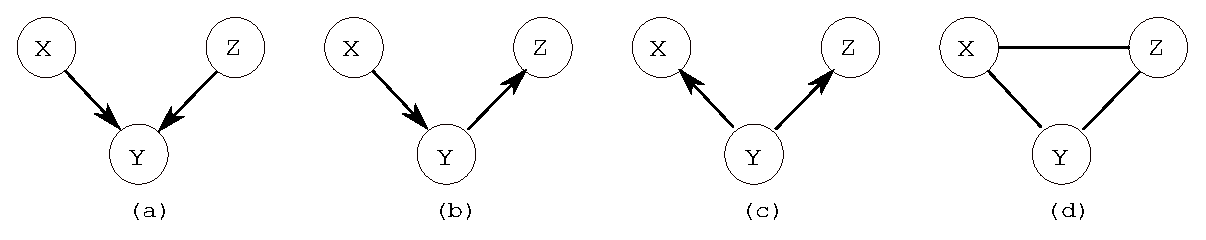
\includegraphics[width=0.80\textwidth]{vstructure.eps}
	\caption{Non-fully connected configurations of 3 variables. See text for details.}
	\label{fig:vstructure}
\end{figure}

Figure \ref{fig:vstructure} shows some configurations of three variables $X,Y$ and $Z$: (a) \emph{Collider} ($X \ci Z$ but $X \dep Z\ |\ Y$), (b) \emph{Chain} ($X \ci Z\ |\ Y$), and (c) \emph{Fork} ($X \ci Z\ |\ Y$). Note that the chain and fork are in the same conditional independence class, but the collider is uniquely specified by its conditional independence properties. The collider is therefore an important structure in causal discovery. In hypothesis tests, such as the prototypical Inductive Causation algorithm \cite[\S 2.5]{06}, colliders are identified by looking for any variables $X$ and $Z$ which are unconnected (dependent under every conditioning set) with each other, but both of which are connected with a third variable $Y$. When such a configuration is found, the edges are orientated as in Figure \ref{fig:vstructure}(a). This is the approach that we adopt here, using the RLVQ framework itself rather than hypothesis tests.

\section{RLVQ}
\label{sec:RLVQ}

The basic LVQ scheme is set up as follows; Given a dataset $D = \left\{\textbf{x}^\mu, y^\mu\right\}^P_{\mu = 1}$ where $\textbf{x}^\mu \in \textbf{R}^N$ and the labels $y^\mu \in {1,2,\ldots C}$ correspond to one of the classes, the LVQ scheme is parameterized by a set of prototype vectors $\textbf{w} = \left\{\textbf{w}^j, c(\textbf{w}^j)\right\}^M_{j=1}$ with the prototype vectors $\textbf{w}^j$ having labels $c(\textbf{w}^j) \in {1,2,\dots C}$.

For a particular dissimilarity/distance measure $d(\textbf{x,w})$, the LVQ classifier employs a Winner-Takes-All scheme where an arbitrary input is assigned to the class $c(\textbf{w}^L)$ of the closest prototype with $d(\textbf{x},\textbf{w}^L) \leq d(\textbf{x},\textbf{w}^j)$ \textsl{for all} $j$.

Many modifications of Kohonen's original formulation \cite{02} have been suggested with the aim of achieving better convergence and generalization behavior. A specific set of modifications have been towards accounting for heterogeneous datasets where features can have different meanings and magnitudes. These are the class of relevance learning schemes which employ adaptive scaling factors for each dimension in the feature space. For our purposes it will suffice to give the general formulation of RLVQ.

For RLVQ we can consider a generalized Euclidean distance of the form
%
\begin{equation} 
d(\textbf{x},\textbf{w}^J) = \sum^N_{j=1} \lambda_j (x_j - w^J_j)^2 ,
\end{equation}
%
\noindent
as the dissimilarity measure where $\lambda_j$ are the adaptive relevance factors. The special case $\lambda_j = 1/N$ for all $j = 1,\ldots N$ is analogous to the original LVQ1 formulation. Each update of the winning prototype $w_j$ is accompanied by a corresponding update in the relevance factor $\lambda_j(t)$ as follows;
%
\begin{equation}
\lambda_j(t) = \lambda_j(t-1) - \eta_\lambda \phi \cdot (x_j - w^J_j)^2  \quad \text{with} \quad
\phi = \begin{cases}
+1& \text{if $y^\mu = c(\textbf{w}^J(t))$},\\
-1& else 
\end{cases}
\end{equation}
%
where $\lambda_j(t)$ is restricted to non-negative values and obeys the normalization $\sum^N_{j=1} \lambda_j = 1$.

The $\lambda$ update hence decreases the relevance factor $\lambda_j$ if the winning prototype $\textbf{w}^J$ does represent the correct class but the contribution $(\textbf{x}_j - \textbf{w}^J_j)^2$ to $d(\textbf{x},\textbf{w}^J)$ is relatively large. Conversely the weight of a feature with relatively small $(\textbf{x}_j - \textbf{w}^J_j)^2$ is increased in such a case. The learning rate $\eta_\lambda$ controls the magnitude of the prototype and relevance factor updates at each step.

\section{Causal RLVQ}
\label{sec:CRLVQ}

CRLVQ is our extension of the RLVQ scheme where updates favor features that are causally related to the target feature. Our assessment of causal relevance is based on identifying V-structures with respect to the target. RLVQ gives a profile that represents how strongly each single dimension of the data is predictive of the target. In CRLVQ instead of looking at a single dimension, we look for evidence that there are two dimensions $x_i$ and $x_k$ that are predictive of the target. To ascertain that $x_i$ and $x_k$ are in a V-structure with the target we also check that they are independent of each other.

\begin{figure}
\begin{tabular}{m{.5\textwidth}cm{.4\textwidth}}
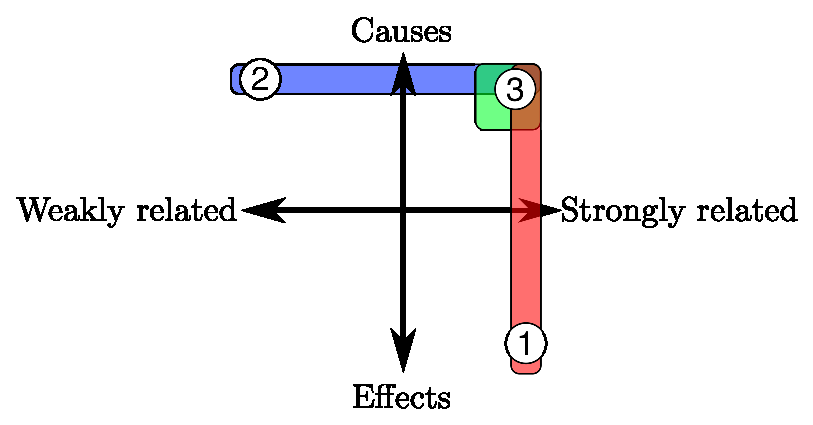
\includegraphics[width=.5\textwidth]{causal-relevance-dimensions.eps} & &
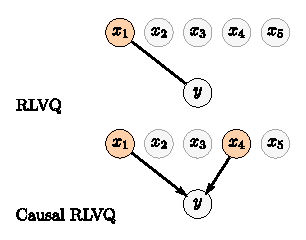
\includegraphics[width=.35\textwidth]{rlvq-crlvq.eps} \\
& \\
(a) & & (b)  
\end{tabular}
\label{fig:causes}
\caption{RLVQ and CRLVQ formulations. Panel (a) is an illustration of placement of variables across the predictive-causal space. Panel (b) shows how RLVQ is extended to CRLVQ}
\end{figure}

Figure 2(a) illustrates this salient distinction between RLVQ and CRLVQ. We conceive of features $(x_1, \ldots, x_P)$ as being characterisable along two dimensions: their predictiveness of the target variable, and their causal effect on the target variable. Standard relevance learning aims to give higher weight to a set of variables (1) which are highly predictive; causal structure learning aims to find causes (2) or effects of a target; our work here identifies variables which are predictive causes (3). Figure 2(b) shows the difference in which RLVQ considers each feature separately; CRLVQ takes features pairwise in order to identify V-structures with the target.
 
CRLVQ extends the RLVQ update by adding two extra evaluation criteria to equation 2. The three criteria in total are in a sense a distance-based formulation of the V-structure condition. For every example presented to the CRLVQ classification scheme, each component of $\lambda$ in CRLVQ is hence updated for every dimension $x_j$ for each introduction of a data example as follows
%
\begin{equation} 
\lambda_j(t) = \lambda_j(t-1) - \eta_\lambda \phi \cdot (x_j - w_j^J)^2 - \alpha \eta_\lambda \cdot \left( \min_{k \neq j}\left(\phi \cdot (x_k - w_k^J)^2 - (x_j - x_k)^2 \right) \right)
\end{equation}
%
The parameter $\alpha$ is a parameter that weights the two new criteria. Standard RLVQ is hence a special case of CRLVQ when $\alpha = 0$. We evaluate the independence of the different data dimensions by looking at their absolute difference. In Z-score transformed data, this will be a small quantity for pairs of dimensions that are positively correlated. The update hence rewards any feature $x_j$ if it has a strong correlation (small difference) with the target/label vector as represented by a correct prototype $(x_j - w_j^J)^2$ , and also if there is strong evidence of another feature with a strong correlation to the target as well $(x_k - w_k^J)^2$, and if feature $x_j$ and $x_k$ are weakly correlated (large difference apart).

Note however that there might be other relationships between the dimensions that make them dependent on each other, but that this update would not capture -- for example negative correlation. 

\section{Experiments}
\label{sec:Experiments}

Simulated causal networks were used to demonstrate the effect of the causal $\lambda$ update. One causal network was formulated as a 5-feature linear Gaussian network with 2 causes, 2 effects and 1 irrelevant feature, shown in Figure 3(a). In Figure 3(b) we can see that as $\alpha$ is increased, the relevance weights increase for the features that are causally relevant. 

\begin{figure}
\begin{tabular}{cc}
\begin{tabular}{c}
\vspace{-3cm} \\ 
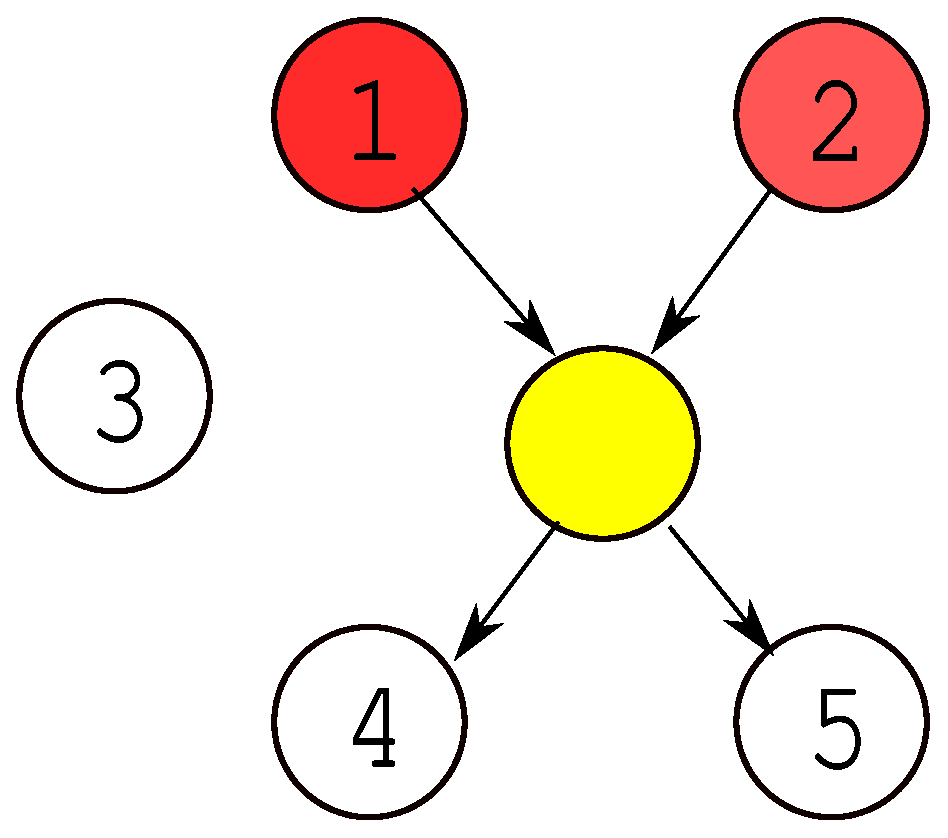
\includegraphics[scale=0.15]{simnetwork.eps} \\
\vspace{1cm} 
\end{tabular} & 
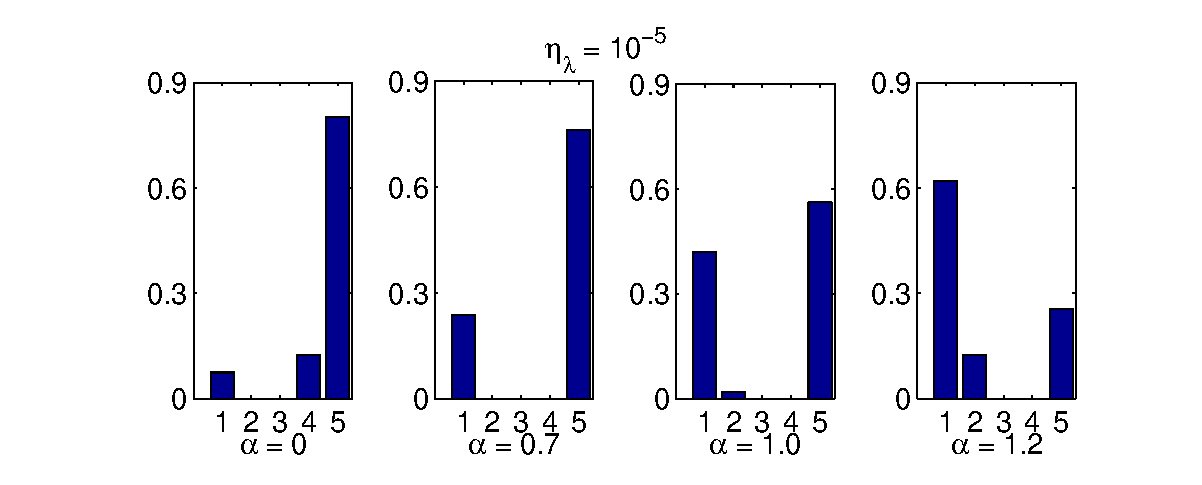
\includegraphics[width=.7\textwidth]{simlambda.eps} \\
(a) &  (b)  
\end{tabular}
\label{fig:simnetwork}
\caption{CRLVQ relevance weights for simulated network data. Panel (a) shows the simulated network with 2 causes, 2 effects and 1 irrelevant feature. Panel (b) shows the relevance profile under RLVQ and under CRLVQ for different parameter settings.}
\end{figure}

For experiments on manipulated test sets we used a network simulated from a Bayes net and used for several causal competitions as a trial set for tuning causal algorithms. It is commonly called the Lucas dataset\cite{12,13} and tries to predict lung cancer based on different features. Three versions of the dataset were used: Lucas0, the natural network (unmanipulated) from which the training set was obtained, and manipulated datasets Lucas1 and Lucas2 (manipulated variables shown in Figure \ref{fig:lucasgraph}). All training was carried out on unmanipulated data. 
\begin{figure}[t]
	\centering
		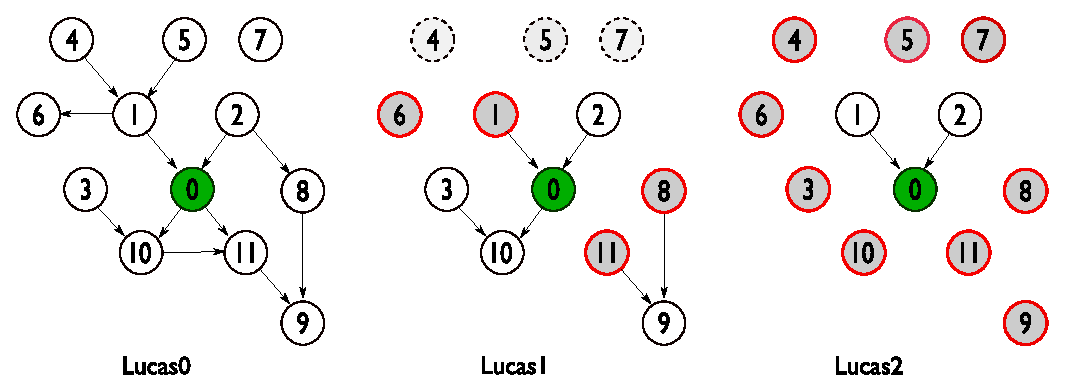
\includegraphics[width=0.8\textwidth]{lucasgraph.eps}
	\caption{\footnotesize{Lucas graphs showing the network structures for the unmanipulated set, Lucas0 and the manipulated sets, Lucas1 and Lucas2. The different features in the graphs are labelled as follows; 0 - Lungcancer, 1 - Smoking, 2 - Genetics, 3 - Allergy, 4 - Anxiety, 5 - Peer Pressure, 6 - Yellow Fingers, 7 - Born an Even Day, 8 - Attention Disorder, 9 - Car Accident, 10 - Coughing, 11 - Fatigue.}}
	\label{fig:lucasgraph}
\end{figure}

Figure \ref{tab:TestErrorResults} shows the test error scores for the three datasets Lucas0, Lucas1 and Lucas2 for CRLVQ with varying $\alpha$ parameters. The first row with $\alpha$ = 0 represents RLVQ. Lucas0 represents the unmanipulated(natural) dataset while Lucas1 and Lucas2 represent manipulated/intervened upon datasets. Test results are obtained after 50 epochs through the data with $\eta_\lambda = 10^{-5}$.

\begin{figure}[t]
	\centering
	\subfloat[Results][Results]{
%\begin{table}
 %\centering
			%\begin{footnotesize}
\begin{tabular}{c}
\vspace{-3.2cm} \\ 
\begin{tabular}{|c|c|c|c|}
\hline
      &         \multicolumn{ 3}{|c|}{Lucas Dataset}   \\
\hline
$\alpha$ &  Lucas0 &     Lucas1 &     Lucas2  \\
\hline
  0    &    0.1970 &     0.2370 &     0.2620  \\
\hline
  1.0 &     0.2040 &     0.2040 &     0.2030  \\
\hline
  2.0 &     0.2040 &     0.2040 &     0.2030   \\
\hline
\end{tabular}
\vspace{0cm}
\end{tabular} }
\subfloat[lucaslambda][RLVQ as $\lambda$ changes]{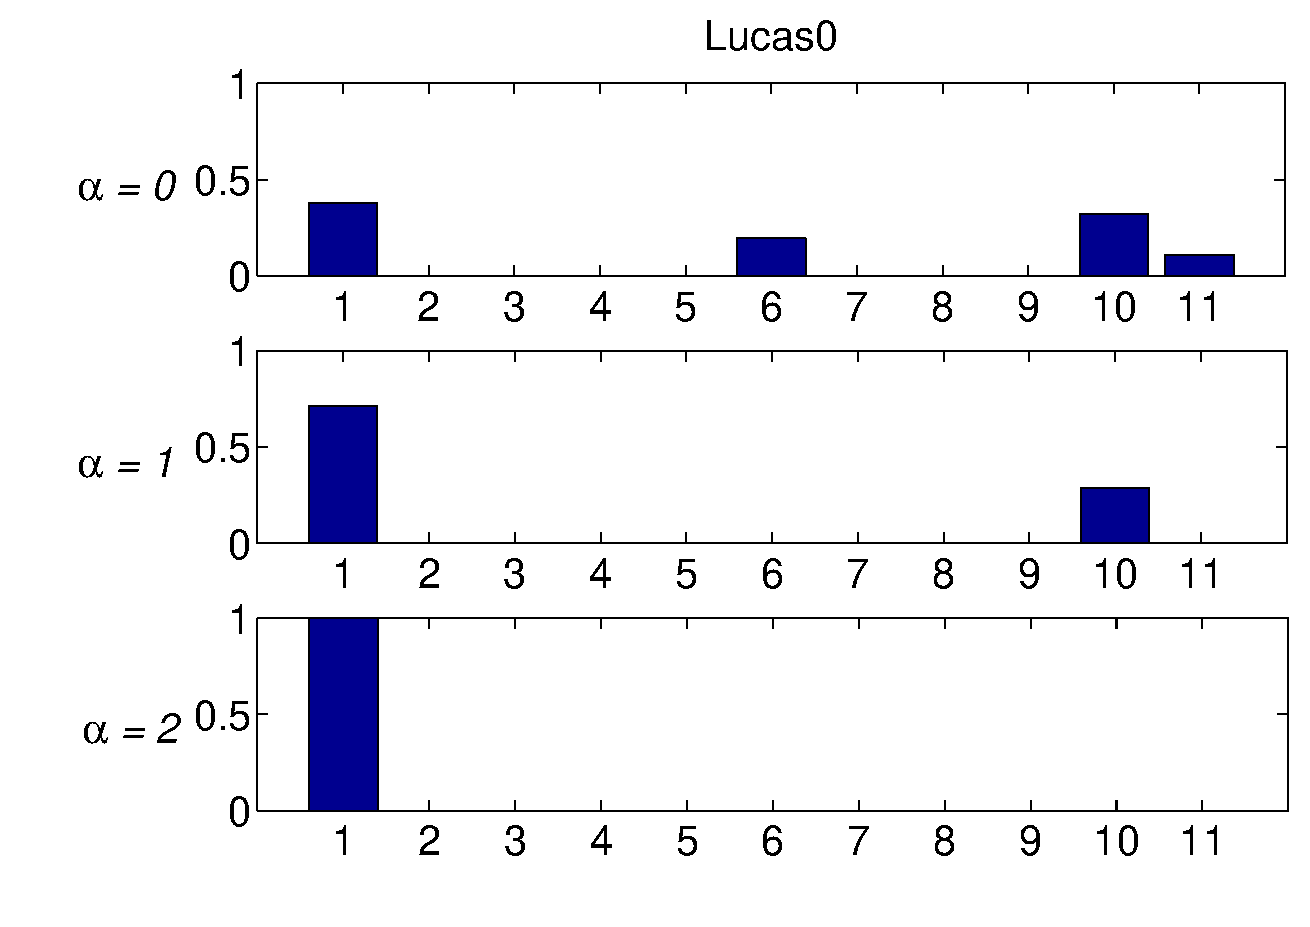
\includegraphics[width=0.5\textwidth]{lucaslambda.eps}}  
			%\end{footnotesize}
	\caption{Test error results for RLVQ and CRLVQ for the different datasets Lucas0, Lucas1 and Lucas2.}
	\label{tab:TestErrorResults}
\end{figure} 

The unmanipulated dataset is best predicted by RLVQ ($\alpha = 0$). For the manipulated datasets, we notice that test error increases for RLVQ as expected because there are fewer relevant features. We also see an increase in performance on these datasets as $\alpha$ is increased, as causal dimensions in the data dominate the distance measure. Figure 5 (b) illustrates the relevance profile for the different values of $\alpha$; we can see that as $\alpha$ increases, the relevance weight of variable 1 (a cause) is increased at the expense of variables 10 and 11 (effects).

%For the manipulated datasets, Lucas1 and Lucas2 we notice the opposite effect. There is better accuracy as $\alpha$ is increased as expected because the causes remain predictive after the data is manipulated. A higher $\alpha$ biases the relevance profile towards causally relevant features hence the increase in performance. While generally this is true, the performance tends to be sensitive to the values of $\alpha$ and the RLVQ learning rate $\eta_\alpha$.

\section{Conclusion}
\label{sec:Conclusion}

This paper applies concepts from causal discovery to relevance learning for prototype-based classification. The goal is to assure robust classification when it is not certain that the test set has the same distribution as the training set.
%Our parameterisation $\alpha$ allows us to adjust the bias towards causative features, where $\alpha=0$ yields standard RLVQ.
We have given a proof of possibility on simulated data, though our formulation still has some limitations, particularly in our assessment of independence amongst features in the data. An interesting direction to address this could be to extend our current work to matrix relevance LQV \cite{09}.

\textbf{Acknowledgement:} We would like to acknowledge funding from NUFFIC Project NPT-UGA-238: Strengthening ICT Training and Research Capacity in Uganda, and from Google, for this work.

% ****************************************************************************
% BIBLIOGRAPHY AREA
% ****************************************************************************

\begin{footnotesize}

\bibliographystyle{unsrt}
\bibliography{esann2011}

\end{footnotesize}

% ****************************************************************************
% END OF BIBLIOGRAPHY AREA
% ****************************************************************************

\end{document}
